\documentclass[11pt,a4paper,titlepage]{article}
\usepackage[brazil]{babel}
\usepackage[utf8]{inputenc}
\usepackage[T1]{fontenc}

\newcommand{\titulo}{\textit{Relatório III - Controle e Memória de Instruções}}

\newcommand{\cabecalho}{\textit{Relatório III}}

\usepackage{fancyhdr}
\usepackage{indentfirst}
\usepackage{setspace}
\usepackage{graphicx,url}
\usepackage[section]{placeins}
%\usepackage{color,colortbl}
\usepackage{amsmath}
\usepackage{amssymb}
\usepackage{amsthm}
\usepackage{wrapfig}
\usepackage{times}
\usepackage{hyphenat}
\usepackage{ae}
\usepackage{algorithm}
\usepackage[sort,numbers]{natbib}
%package to insert codes
\usepackage{listings}
\usepackage{mips}
\usepackage{tabularx}
\usepackage{makecell}
%appendix
\usepackage[titletoc,toc,page]{appendix}
\renewcommand{\appendixtocname}{Apêndices}
\renewcommand{\appendixpagename}{Apêndices}

% the following is needed for syntax highlighting
\usepackage{color}

\definecolor{dkgreen}{rgb}{0,0.6,0}
\definecolor{gray}{rgb}{0.5,0.5,0.5}
\definecolor{mauve}{rgb}{0.58,0,0.82}

\lstset{ %código assembly
  language=[mips]Assembler,       % the language of the code
  basicstyle=\footnotesize,       % the size of the fonts that are used for the code
  numbers=left,                   % where to put the line-numbers
  numberstyle=\tiny\color{gray},  % the style that is used for the line-numbers
  stepnumber=1,                   % the step between two line-numbers. If it's 1, each line 
                                  % will be numbered
  numbersep=5pt,                  % how far the line-numbers are from the code
  backgroundcolor=\color{white},  % choose the background color. You must add \usepackage{color}
  showspaces=false,               % show spaces adding particular underscores
  showstringspaces=false,         % underline spaces within strings
  showtabs=false,                 % show tabs within strings adding particular underscores
  frame=single,                   % adds a frame around the code
  rulecolor=\color{black},        % if not set, the frame-color may be changed on line-breaks within not-black text (e.g. commens (green here))
  tabsize=4,                      % sets default tabsize to 2 spaces
  captionpos=b,                   % sets the caption-position to bottom
  breaklines=true,                % sets automatic line breaking
  breakatwhitespace=false,        % sets if automatic breaks should only happen at whitespace
  title=\lstname,                 % show the filename of files included with \lstinputlisting;
                                  % also try caption instead of title
  keywordstyle=\color{blue},          % keyword style
  commentstyle=\color{dkgreen},       % comment style
  stringstyle=\color{mauve},         % string literal style
  escapeinside={\%*}{*)},            % if you want to add a comment within your code
  morekeywords={*,...}               % if you want to add more keywords to the set
}
\usepackage{xcolor}
\definecolor{vgreen}{RGB}{104,180,104}
\definecolor{vblue}{RGB}{49,49,255}
\definecolor{vorange}{RGB}{255,143,102}
%mostrar código do verilog
\lstdefinestyle{verilog-style}
{
    language=Verilog,
    basicstyle=\small\ttfamily,
    keywordstyle=\color{vblue},
    identifierstyle=\color{black},
    commentstyle=\color{vgreen},
    numbers=left,
    numberstyle=\tiny\color{black},
    numbersep=10pt,
    tabsize=8,
    moredelim=*[s][\colorIndex]{[}{]},
    literate=*{:}{:}1
}

\makeatletter
\newcommand*\@lbracket{[}
\newcommand*\@rbracket{]}
\newcommand*\@colon{:}
\newcommand*\colorIndex{%
    \edef\@temp{\the\lst@token}%
    \ifx\@temp\@lbracket \color{black}%
    \else\ifx\@temp\@rbracket \color{black}%
    \else\ifx\@temp\@colon \color{black}%
    \else \color{vorange}%
    \fi\fi\fi
}
\makeatother

\usepackage{trace}

% Criar figura dividida em subfiguras
\usepackage{subfigure}

\usepackage{subfig}
\usepackage{ae}
\usepackage{aecompl}

\usepackage{multirow}
%\usepackage{epstopdf}

\pagestyle{fancy}

\setlength{\evensidemargin}{0.0in}
\setlength{\oddsidemargin}{0.0in}
\setlength{\textwidth}{6.6in}
\setlength{\textheight}{1.06\textheight}

\lhead{}
\chead{}
\rhead{\footnotesize{\textsc{\cabecalho}}}
\lfoot{\footnotesize{Guilherme Batista Santos, Iuri Silva Castro, João Mateus de Freitas Veneroso, Ricardo Pagoto Marinho}}
\cfoot{}
\rfoot{\footnotesize{\thepage}}
\setlength{\headwidth}{\textwidth}
\renewcommand{\headrulewidth}{0.4pt}
\renewcommand{\footrulewidth}{0.4pt}
\renewcommand{\baselinestretch}{0.90}

%\hyphenation{ ca-rac-te-ri-zan-do--se }

\begin{document}

\begin{titlepage}
\begin{center}

\begin{large}
Universidade Federal de Minas Gerais\\
Instituto de Ciências Exatas\\
Departamento de Ciência da Computação\\
\end{large}

\vspace{20mm}

\begin{Large}
DCC819 - Arquitetura de Computadores
\end{Large}

\vspace{20mm}

\begin{LARGE}
\titulo
\end{LARGE}


\vspace{30mm}

\begin{Large}
\begin{center}
Guilherme Batista Santos\\ Iuri Silva Castro\\ João Mateus de Freitas Veneroso\\ Ricardo Pagoto Marinho \\
\end{center}
\end{Large}


\vspace{60mm}

{\sc Belo Horizonte - MG}

{\sc \today}

%\vspace{10mm}
\end{center}
\end{titlepage}


\section{Descrição}\label{sec:desc}

Deseja-se, agora, que o microprocessador seja capaz de ler instruções de uma memória de instruções e que as execute que forma sequencial. Instruções de controle de fluxo como \textit{BEZ (Branch if Equals Zero)} e \textit{J (Jump)} são necessárias para o controle de execução dos programas. Para tais tarefas necessita-se de um sistema de controle robusto, mais complexo do que o anteriormente implementado. 

Para a validação do sistema utilizou-se de um algoritmo de ordenação de números inteiros positivos. Viu-se a necessidade de implementar a instrução \textit{SLT Reg-Reg}, para fazer a comparação entre registros, anteriormente implementada apenas a versão imediatada ta instrução (SLTI Reg-Imm).

\section{Implementação}

Para atender as requisições, fez-se a modificação de vários módulos já implementados em relatórios passados.
Adicionado instrução de SLT Reg-Reg.

O único módulo que permanenceu inalterado é o do banco de registradores.



\subsection{Memória de Instruções}\label{subsec:imp-instmemory}

A memória de instruções é uma memória do tipo ROM (Read-Only Memory).

\begin{figure}[!h]
\centering
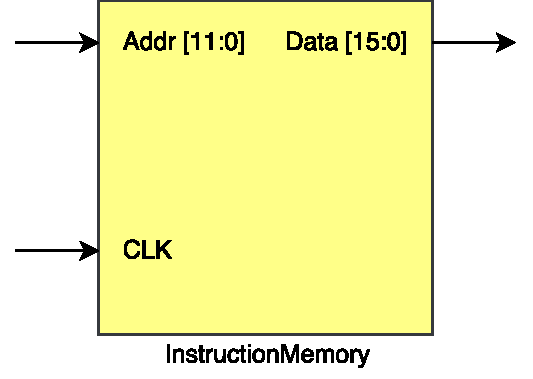
\includegraphics[scale=0.4]{images/InstructionMemory.pdf}
\caption{Módulo da Memória de Instruções.}
\label{fig:instrmemory}
\end{figure}



\subsection{Decodificador}\label{subsec:imp-decode}

O decodificador mantem o registrador de instruções (Instruction Register, IR), que mantem a instrução que está sendo atualmente executada.

\begin{figure}[!h]
\centering
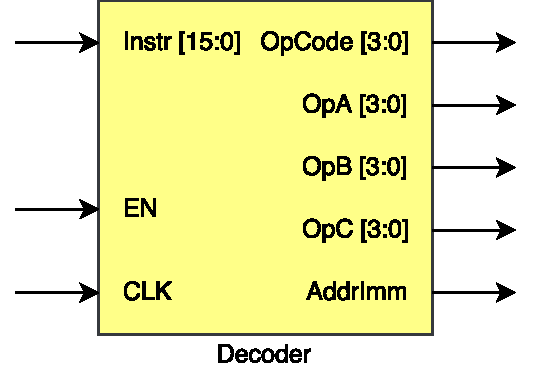
\includegraphics[scale=0.4]{images/Decoder.pdf}
\caption{Módulo de decodificação.}
\label{fig:decoder}
\end{figure}

\subsection{ULA}\label{subsec:imp-ula}

Para o módulo da ULA, implementou-se a operação de BEZ, onde ela compara o valor do operando A com zero (OpA == 0?), retornando como resultado o valor do operando B (res = OpB) e ajustando o campo Zero do registro de flags de acordo com a comparação. Modificou-se também a ULA para que ela seja completamente combinacional, não havendo mais registros e nem sincronização com o sinal de clock.

\begin{figure}[!h]
\centering
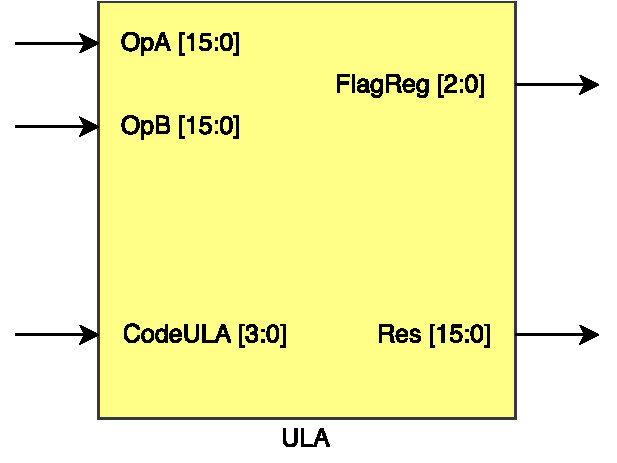
\includegraphics[scale=0.4]{images/ULA.pdf}
\caption{Unidade Lógica Aritmética.}
\label{fig:ula}
\end{figure}

\subsection{Controle}\label{subsec:imp-ctrl}

Estágios da máquina de controle. Sinais de controle adicionados, sinais de controle não utilizados.

\begin{figure}[!h]
\centering
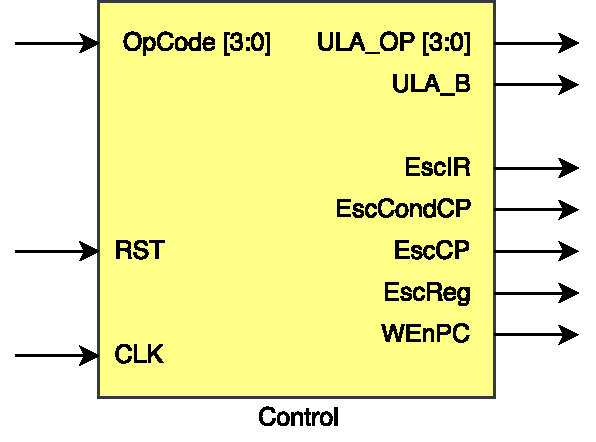
\includegraphics[scale=0.4]{images/Control.pdf}
\caption{Módulo de controle.}
\label{fig:control}
\end{figure}

\section{Integração}

Mux's para seleção de PC. Adder externo para incremento de PC. Considerar que os sinais de clock (CLK) e reset (RST) são globais, e estão conectados em todos os módulos que os têm. O diagrama do sistema pode ser visto na figura \ref{fig:microprocessor}.

\begin{figure}[h]
\centering
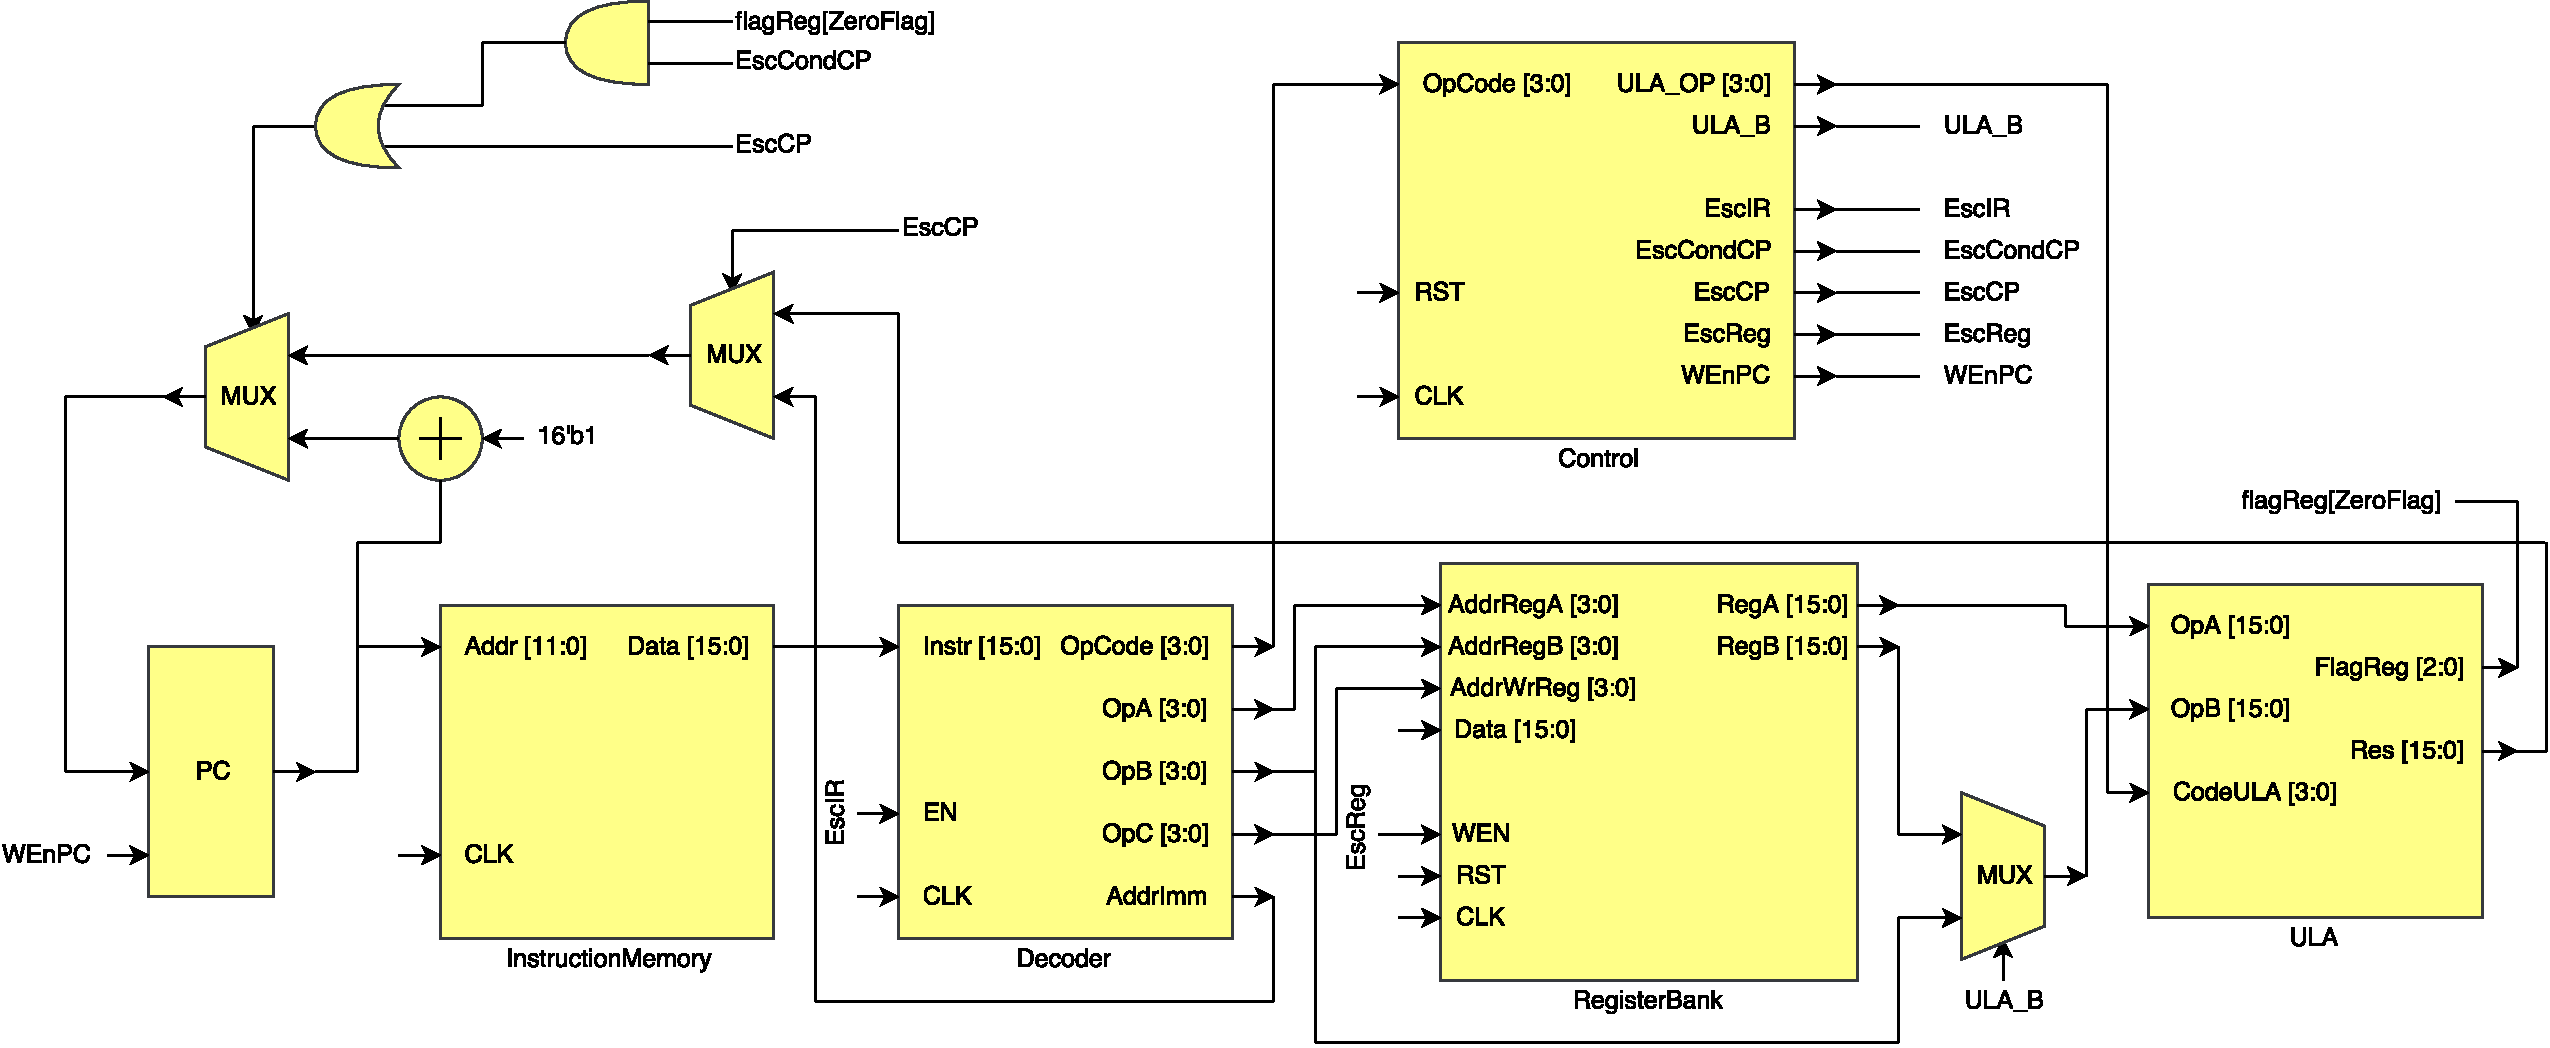
\includegraphics[scale=0.4]{images/Microprocessor.pdf}
\caption{Sistema completo e conexões.}
\label{fig:microprocessor}
\end{figure}

\section{Simulação e Testes}

Integrado o microprocessador passa-se para o processo de simulação e teste para validar a implementação. Para tal, gerou-se um algoritmo para fazer a ordenação de um vetor, utilizando os registros R11, R12, R13, R14 e R15 como elementos do vetor. O algoritmo faz a ordenação de forma decrescente, colocando o elemento de maior valor em R11 e o de menor valor em R15, trabalhando apenas com valores inteiros positivos.

\lstset{language=[mips]Assembler}
\begin{lstlisting}
START:
    XOR   R8, R8, R8    // Zera contador de swaps
    SLT   R10, R11, R12   
    BEZ   N0SWAP1, R10
    ADDI  R10, 0, R11
    ADDI  R11, 0, R12
    ADDI  R12, 0, R10
    ADDI  R8, 1, R8     // Incrementa contador de swaps
NOSWAP1:
    SLT   R10, R12, R13
    BEZ   N0SWAP2, R10
    ADDI  R10, 0, R12
    ADDI  R12, 0, R13
    ADDI  R13, 0, R10
    ADDI  R8, 1, R8     // Incrementa contador de swaps
NOSWAP2:
    SLT   R10, R13, R14
    BEZ   N0SWAP3, R10
    ADDI  R10, 0, R13
    ADDI  R13, 0, R14
    ADDI  R14, 0, R10
    ADDI  R8, 1, R8     // Incrementa contador de swaps
NOSWAP3:
    SLT   R10, R14, R15
    BEZ   TEST, R10
    ADDI  R10, 0, R14
    ADDI  R14, 0, R15
    ADDI  R15, 0, R10
    ADDI  R8, 1, R8     // Incrementa contador de swaps
TEST:
    BEZ   END, R8       // Teste se houve algum swap
    J     START         // Houve, retornar para inicio
END:
    J     end           // Fim de execucao, loop infinito
\end{lstlisting}

A instrução BEZ (Branch if Equals Zero) requer que o ponteiro para qual o programa será desviado caso ocorra o branch seja armazenado em um registrador. Assim, precisa-se calcular a posição das labels do programa e carregar tais valores no banco de registradores durante a inicialização do programa. A tabeka abaixo relaciona os labels com suas posições e registros.

\begin{table}[h]
\centering
\begin{tabular}{| c | c | c |}
\hline
Label & Posição & Registro\\
\hline
START & 0 & -\\
\hline
NOSWAP1 & 7 & R1\\
\hline
NOSWAP2 & 13 & R2\\
\hline
NOSWAP3 & 19 & R3\\
\hline
TEST & 25 & R4\\
\hline
END & 27 & R5\\
\hline
\end{tabular}
\caption{Labels e posições na memória de instrução.}
\label{tab:labels}
\end{table}
\captionsetup{font={footnotesize,rm},justification=centering,labelsep=period}%

Não atribui-se registro ao label \textit{START} pois não há instrução \textit{BEZ} que faz desvio desvio para sua posição, apenas instrução \textit{J} que utiliza imediato ao invés de ponteiro.

Converteu-se o código assembly para binário, para que então possa ser gravado no arquivo de inicialização de memória (.mif).

\begin{lstlisting}
0101100010001000
1101101010111100
1100000000011010
1001101000001011
1001101100001100
1001110000001010
1001100000011000
1101101011001101
1100000000101010
1001101000001100
1001110000001101
1001110100001010
1001100000011000
1101101011011110
1100000000111010
1001101000001101
1001110100001110
1001111000001010
1001100000011000
1101101011101111
1100000001001010
1001101000001110
1001111000001111
1001111100001010
1001100000011000
1100000001011000
1011000000000000
1011000000011011
\end{lstlisting}



\section{Discussões}

Houve-se problemas para conseguir simular corretamente o módulo de memória no software ModelSim, principlamente problemas relacionados com o arquivo de inicialização de memória (.mif). Para contornar tais problemas, modificou-se o arquivo "InstrMemory.v", colocando o caminho completo do arquivo de inicialização. Pede-se ao leitor que ao fazer a reprodução da simulação atente-se a esse detalhe e que faça a modificação do caminho do arquivo para atender às configurações da máquina em que está trabalhando.
Devido as limitações das formas de endereçamento atual da máquina, é necessário calcular os ponteiros dos labels ao qual os branches farão o salto no programa, armazenando-os anteriormente no banco de registradores.

%%%%%%%%%%%%%%%%%%%%%%%%%%%%%%%%%%%%%%%%%%%%%%%%%%%%%%%%%%%%%%%%%%%%%%%%%%%%%%%%%%%%%%%%%%%%%%%%%%%%%%%%%%%%%%%%%%%%%%%%%%%%%%%%%%%
% Para mudar o nome da seo de referncias
%\renewcommand{\bibname}{Referncias}
%\renewcommand{\refname}{Referncias}

\bibliographystyle{unsrt}
\addcontentsline{toc}{section}{Referências}
%\bibliography{references}

\nocite{*}


\end{document}

